\newpage
\section{A Large Ion Collider Experiment at the LHC}
ALICE (A Large Ion Collider Experiment) has been collecting data during the whole first phase of the Large Hadron Collider operations, from its startup on the 23 November 2009 to the beginning of the first long technical shutdown in February 2013. During the first three years of operations LHC provided pp collisions at 0.9, 2.76, 7 and 8 TeV, Pb--Pb collisions at 2.76A TeV and finally p--Pb collisions at 5.02 TeV. The first section of this chapter focuses on the LHC performance during this phase and includes details on the accelerator parameters that allow the LHC to perform as a lead ion collider. A detailed description of the ALICE detector follows in the section \ref{label:alice}. ALICE has been designed and optimized to study the high particle-multiplicity environment of ultra-relativistic heavy-ion collisions and its tracking and particle identification performance in Pb--Pb collisions are discussed. The attention is drawn in particular on the central barrel detectors. Section \ref{label:aliceDAQ} describes the ALICE Data Acquisition (DAQ) system, that also embeds tools for the online Data Quality Monitoring (DQM). The final part of the chapter is dedicated to the offline computing and reconstruction system based on the GRID framework.


\subsection{The Large Hadron Collider}
The Large Hadron Collider (LHC) \cite{cite:LHC} at CERN is the biggest particle accelerator world-wide. The LHC project was approved in 1994 and construction works in the existing underground tunnel started in 2001 after the dismantling of the LEP collider, which had previously been built in the tunnel which is located under the Swiss-French border area close to Geneva at a depth of 50 to 175 m. The LHC has a circumference of 26.7 km. By design, its maximum achievable energies are 7 TeV for beam of protons and 2.76 TeV per nucleon for beam of lead ions, thus providing collisions at \s = 14 TeV and \snn = 5.5 TeV, respectively. These would be the largest energies ever achieved in particle collision experiments.
The LHC is a synchrotron that accelerates two counter-rotating beams in separate parallel beam pipes. In each of them bunches of particles travel many times around the accelerator ring before the collision energy is reached. The accelerator has to bend the beams around the ring, keep the bunches focused and accelerate them to their collision energy. Finally, the spatial dimension of the bunches has to be minimized in order to attain high luminosity, which ensure a high number of collisions per time interval at the collision points, i.e. a high luminosity. A combination of magnetic and electric field components performs the mentioned tasks. Despite the high luminosity reached, only a very small fraction of the particles of two bunches collides in a single bunch crossing. The others leave the interaction region essentially uninfluenced, are defocused, and continue to circulate in the accelerator.

\begin{figure}[htbp]
\begin{center}
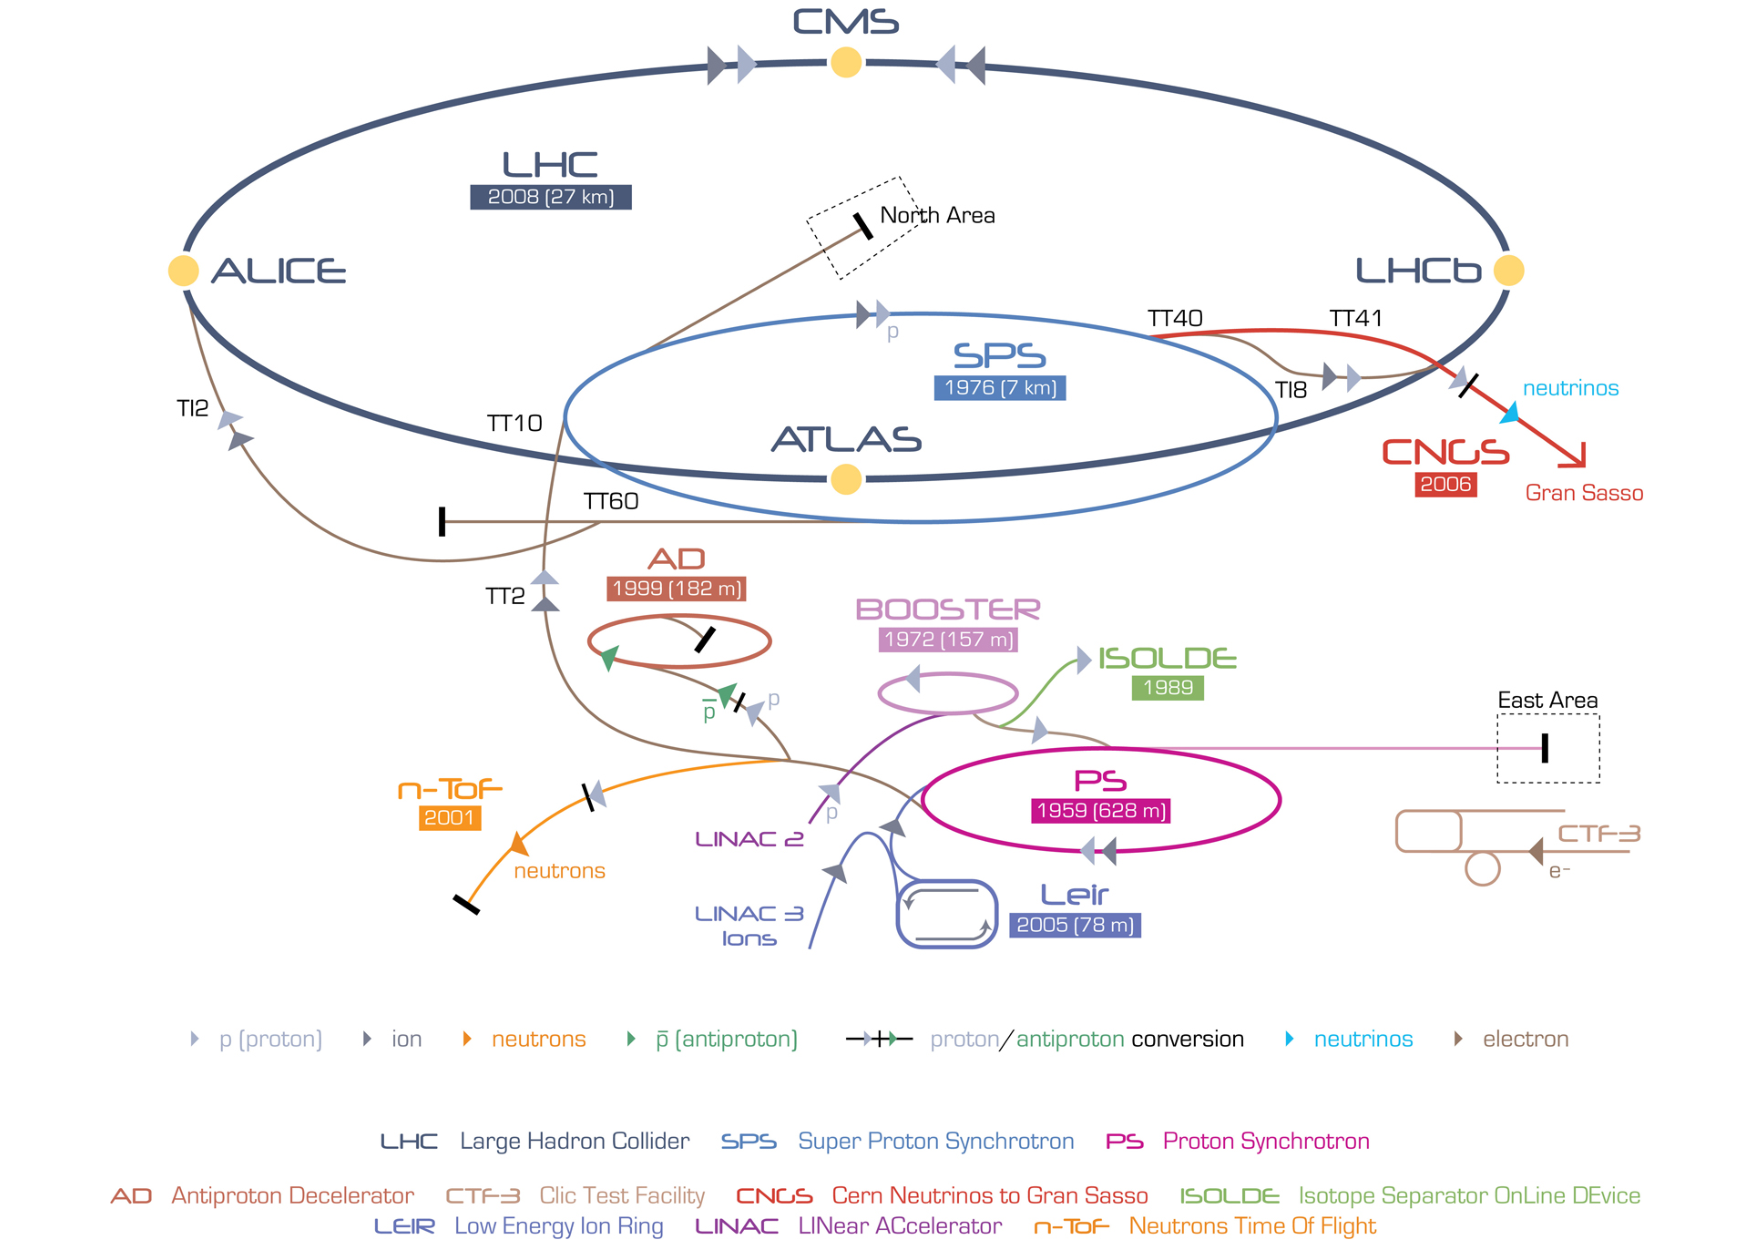
\includegraphics[width=12.cm]{./Version1/FigChapter4/FigureLHC}
\caption{ The CERN accelerator complex \cite{cite:LHCfig}}
\label{fig:lhc}
\end{center}
\end{figure}

Injection of bunches into the LHC (Figure \ref{fig:lhc}) is preceded by acceleration in the LINAC2, PS booster, PS, and SPS accelerators. The acceleration sequence is slightly different for heavy-ions, in which case bunches pass the LINAC3, LEIR, PS, and SPS accelerators (more information can be found in [90]). Several injections to the LHC are needed until all bunches of both beams are filled.
The first pp collisions at 900 GeV centre-of-mass energy were delivered by the LHC on September 10th 2008. Nine days later, the operations were interrupted due to a failure in an electrical connection between two magnets. The machine operators spent over a year repairing and consolidating the accelerator. On November 20th 2009 low energy proton beams circulated again, and a few days later, by achieving the energy of 1.18 TeV per proton beam, LHC became the most powerful accelerator in the world. The first pp collisions at centre-of-mass energy of 7 TeV were delivered in March 2010, and the first Pb?Pb collisions at centre-of-mass energy of 2.76 TeV per nucleon pair in November 2010. In 2010 the integrated luminosity delivered by the LHC was $\sim$ 48 $pb^{-1}$ for pp collisions at \s = 7 TeV ($\sim$ 0.5 $pb^{-1}$ in ALICE) and $\sim$ 10 $\mu b^{-1}$ for Pb?Pb at \snn = 2.76 TeV ($\sim$ 10 $\mu b^{-1}$ in ALICE). In 2011 the beam energy was the same as in 2010 both for pp and Pb--Pb. The performance of the LHC improved in terms of luminosity with $\sim$ 5.61 $fb^{-1}$ for pp ($\sim$ 2 $pb^{-1}$ in ALICE) and $\sim$ 166 $\mu b^{-1}$ for Pb--Pb collisions ($\sim$ 143.62 $\mu b^{-1}$ in ALICE). In 2012, the centre-of-mass energy for pp collisions was brought to 8 TeV and the integrated luminosity (up to December 2012, end of the pp program) was $\sim$ 23.3 $fb^{-1}$ ($\sim$ 10 $pb^{-1}$ in ALICE). A pilot p--Pb run operated at \snn = 5.02 TeV on September 2012, followed by a long p--Pb run on February 2013 with a delivered luminosity of 31.2 $nb^{-1}$. A very short pp run at \s = 2.76 TeV ended the Run1 of the LHC program, marking the start of the first long shutdown (LS1) until the end of 2014. Despite its excellent performance, the LHC has not yet achieved the nominal parameters (\s, $L$), that is the main goal for the next ignition of the machine in 2015. The LHC produces collisions in four so called Interaction Points (IPs) in correspondence of which are located six detectors of different dimensions and with different goals, all able to study the products of the interactions. These are: \\


\textbf{ALICE (A Large Ion Collider Experiment-IP$_{2}$)} \cite{cite:proposalALICE} is a dedicated heavy-ion ex- periment designed to study strongly-interacting matter at very high energy density. It explores the phase transition to the QGP, its phase diagram, and its properties. Furthermore, ALICE will also study collisions of protons, on one hand as a baseline for heavy-ion measurements and on the other hand it contributes to measurements of identified particles by making use of its excellent particle identification capability and its acceptance at very low transverse momenta. \\

\textbf{ATLAS (A Toroidal LHC ApparatuS-IP$_{1}$)} and \textbf{CMS (Compact Muon Solenoid - IP$_{5}$) }\cite{cite:proposalATLAS}\cite{cite:proposalCMS} are general-purpose detectors for pp collisions that are built to cover the widest possible range of physics at the LHC. Specific topics are the search for the Higgs boson and physics beyond the Standard Model, e.g. new heavy particles postulated by supersymmetric extensions (SUSY) of the Standard Model and evidence of extra dimensions.\\

\textbf{LHCb (The Large Hadron Collider beauty experiment-IP$_{8}$)} \cite{cite:proposalLHCb} is a dedicated experiment for the study of heavy flavor physics at the LHC. In particular, the experiment focuses on the study of CP violation and rare decays of beauty and charm particles, to test the Standard Model and to search for evidence of New Physics. The LHCb physics program is complementary to the flavor physics studies conducted at the B-factories and to the direct searches for new particles performed at ATLAS and CMS. \\

\textbf{LHCf (Large Hadron Collider forward experiment-IP$_{1}$)} \cite{cite:proposalLHCf} measures forward particles created during LHC collisions to provide further understanding of high energy cosmic rays. The detector is placed close to the ATLAS experiment. \\

\textbf{TOTEM (TOTal Elastic and diffractive cross-section Measurement-IP$_{5}$)} \cite{cite:proposalTOTEM} measures the total cross-section, elastic scattering, and diffractive processes. The detector is located close to the CMS experiment. \\

\subsection{The ALICE project}
The ALICE experiment at the LHC \cite{cite:ALICE} has as main goal the study of nuclear matter under extreme conditions of temperature and energy density such as those reached in ultra-relativistic heavy-ion collisions. The aim is to verify the QCD prediction of the existence of a phase transition from the common hadronic matter to the Quark-Gluon Plasma. Since ALICE is the only LHC experiment specifically designed for Pb--Pb collisions, it has to be able to cope with the large multiplicities associated with these collision systems and at the same time has to cover as many QGP-related observables as possible. ALICE is also interested in the study of pp interactions, as these are crucial for a comparison with Pb--Pb collisions, to tune Monte Carlo models and per se, like the other LHC experiments. With respect to these experiments, ALICE is endowed with an excellent Particle IDentification (PID) performance, obtained combining different PID techniques from different detectors that are optimized in different momentum ($\ensuremath{p}$) regions.

\subsubsection{ALICE detector}\label{label:alice}
ALICE is a complex of 14 detector subsystems (Figure \ref{fig:alicedetector}) that can be classified in three groups: \\

\textbf{Central detectors} are housed in a solenoid magnet which provides the experiment with a 0.5 T magnetic field and covers the pseudo-rapidity interval -0.9 $< \eta <$0.9 (corresponding to a polar acceptance $\pi$/4 $< \theta <$ 3$\pi$/4). The azimuthal   acceptance is 2$\pi$. They are mainly dedicated to vertex reconstruction, tracking, particle identification and momentum measurement. Starting from the interaction region and going outward, we find the following detectors: 
\begin{itemize}
\item Inner Tracking System (ITS)
\item Time Projection Chamber (TPC)
\item Transition Radiation Detector (TRD)
\item Time Of Flight (TOF)
\end{itemize}


In the mid-rapidity region there are also three detectors with limited azimuthal acceptance: 
\begin{itemize}
\item High Momentum Particle Identification Detector (HMPID)
\item PHOton Spectrometer (POHS)
\item ElectroMagnetic CALorimeter (EMCAL)
\end{itemize}


\textbf{Muon spectrometer} is placed in the forward pseudo-rapidity region (-4.0 $< \eta <$ -2.5) and consists of a dipole magnet and tracking and trigger chambers. It is optimized to reconstruct heavy quark resonances (such as J/$\Psi$ through their $\mu^{+}\mu^{-}$ decay channel) and single muons. \\

\textbf{Forward detectors} are placed in the high pseudo-rapidity region (small angles with respect to the beam pipe). They are small and specialized detector systems used for triggering or to measure global event characteristics. They are:

\begin{itemize}
\item Time Zero (T0) to measure the event time with precision of the order of tens of picoseconds, as needed by TOF
\item VZERO (V0) to reject the beam-gas background and to trigger minimum bias events
\item Forward Multiplicity Detector (FMD) to provide multiplicity information over a large fraction of the solid angle (-3.4 $< \eta <$ -1.7 and 1.7 $< \eta <$ 5)
\item Photon Multiplicity Detector (PMD) to measure the multiplicity and the spatial distribution of photons on an event-by-event basis in the 2.3 $< \eta <$ 3.7 region
\item Zero Degree Calorimeter (ZDC) to measure and trigger on the impact parameter. The ZDC consists of two calorimeters, one for neutrons (ZDC:ZN) and one for protons (ZDC:ZP), and includes also an electromagnetic calorimeter (ZEM)
\end{itemize}

\begin{figure}[htbp]
\begin{center}
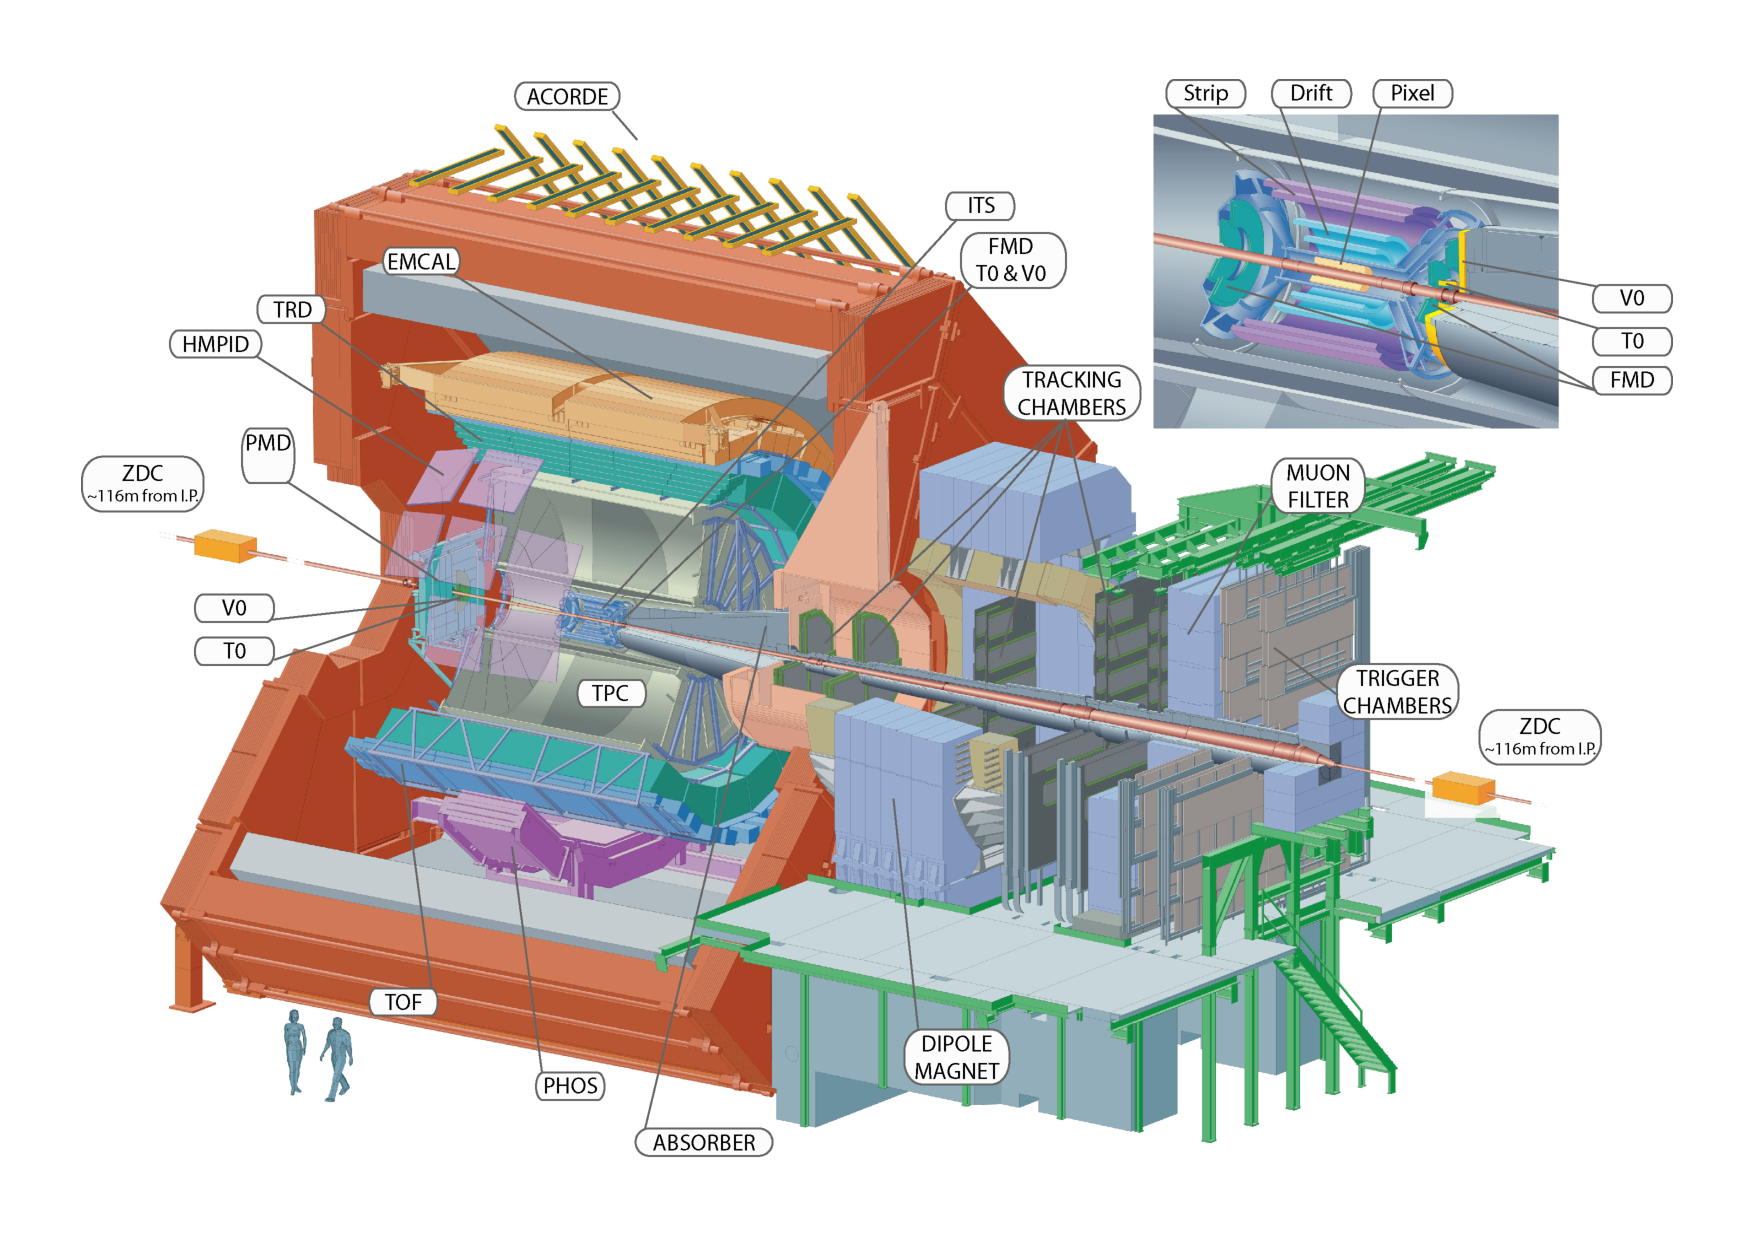
\includegraphics[width=14.cm]{./Version1/FigChapter4/FigureALICE}
\caption{ The ALICE detector}
\label{fig:alicedetector}
\end{center}
\end{figure}


The ALICE global coordinate system \cite{cite:ALICEcoord} is a right-handed orthogonal Cartesian system with the origin X, Y, Z = 0 at the centre of the detector. The three Cartesian axes are defined as follows: the X axis pointing towards the centre of the LHC, the Y axis pointing upward and the Z axis parallel to the local mean beam line pointing in the direction opposite to the muon spectrometer. The azi- muthal angle increases counter-clockwise from the positive X axis ( $\Phi$= 0) to the positive Y axis (  $\Phi$ = $\pi$/2) with the observer standing at positive Z and looking at negative Z; the polar angle increases from the positive Z axis ($\theta$ = 0) to the X-Y plane ($\theta$ = $\pi$/2) and to the negative Z axis ($\theta$ = $\pi$).

In the following Sections more specific descriptions of the detectors used in the identification of the \xis baryons and in the determination of the characteristics of typical collisions will be given. \\

{\Large\textsl{ITS}}\\
The ITS \cite{cite:ALICE} (Figure \ref{fig:its}) is the barrel detector closest to the beam pipe. Its main goals are:
\begin{figure}[htbp]
\begin{center}
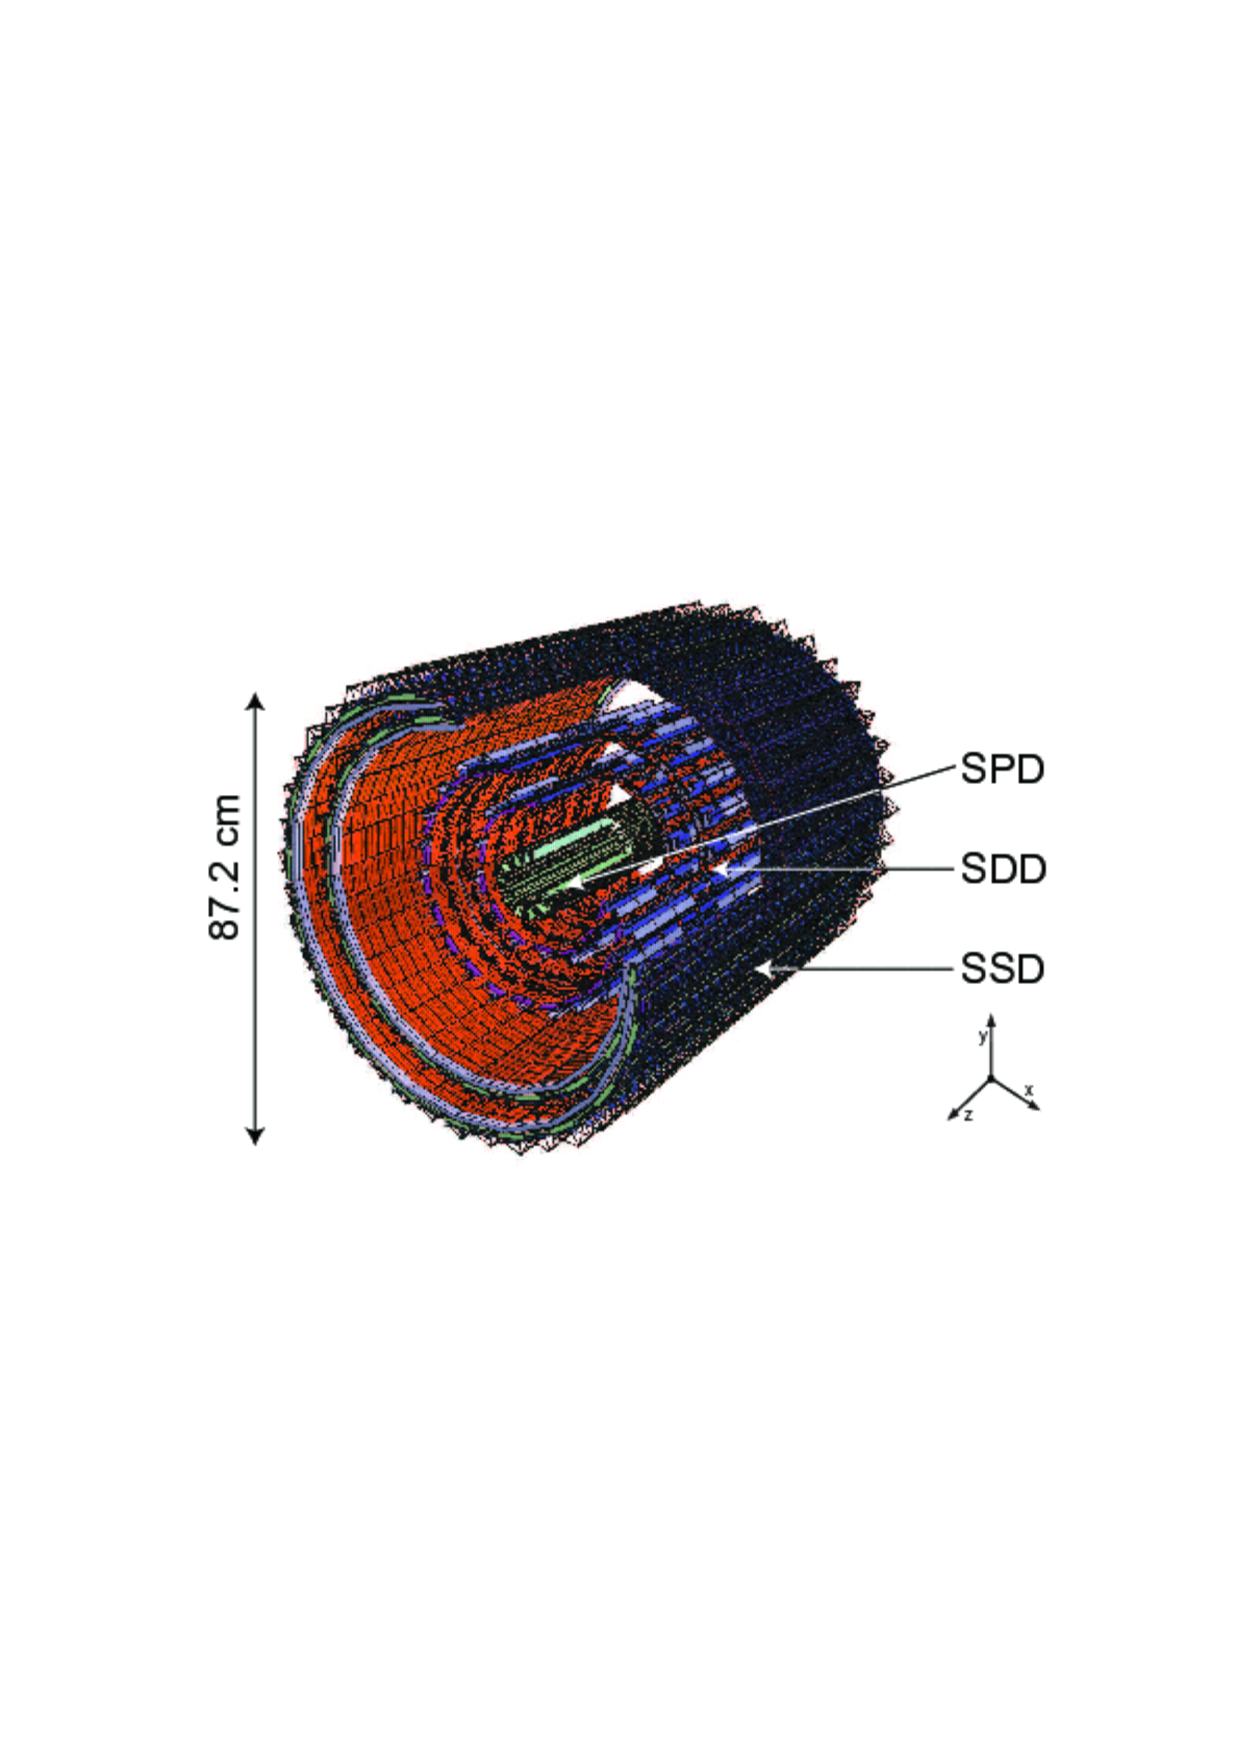
\includegraphics[width=12.cm]{./Version1/FigChapter4/FigureITS}
\caption{Schematic view of the ITS \cite{cite:ITS}}
\label{fig:its}
\end{center}
\end{figure}

\begin{itemize}
\item to contribute with the TPC to the global tracking of ALICE by improving the angle and momentum resolution
\item to reconstruct the position of the primary interaction vertex
\item to reconstruct secondary vertices from decays of heavy-flavor and strange particle decays;
\item to track and identify particles with momentum below 100 \mmass
\item to improve the momentum, impact parameter and angle resolution for the measurement of high \pt particles performed with the TPC
\item to reconstruct particles traversing dead regions of the TPC
\end{itemize}



The ITS surrounds the beam pipe (which is a 800 $\mu$m thick cylinder with an outer diameter of 2.9 cm) and consists of six cylindrical layers of silicon detectors located at radii between 4 cm and 43 cm. Due to the high track density, the two innermost layers are Silicon Pixel Detectors (SPD) which guarantee a high granularity. They are followed by two layers of Silicon Drift Detectors (SDD), while the two outmost layers are double-sided Silicon micro-Strip Detectors (SSD). 




Since the momentum and impact parameter resolutions for low momentum particles are dominated by multiple scattering effects, the amount of material in the active volume has been minimized as much as possible. The granularity of the detector was optimized to keep the occupancy low in all the layers. With the technology chosen, the ITS detectors reach a spatial resolution of the order of a few tens of ?m4 resulting in a resolution on the impact-parameter5 better than 70 ?m in the r  plane for pT > 1 GeV/c and thus well suited for the reconstruction of heavy-flavor decays (see Figure \ref{fig:itsperformance}).

\begin{figure}[htbp]
\begin{center}
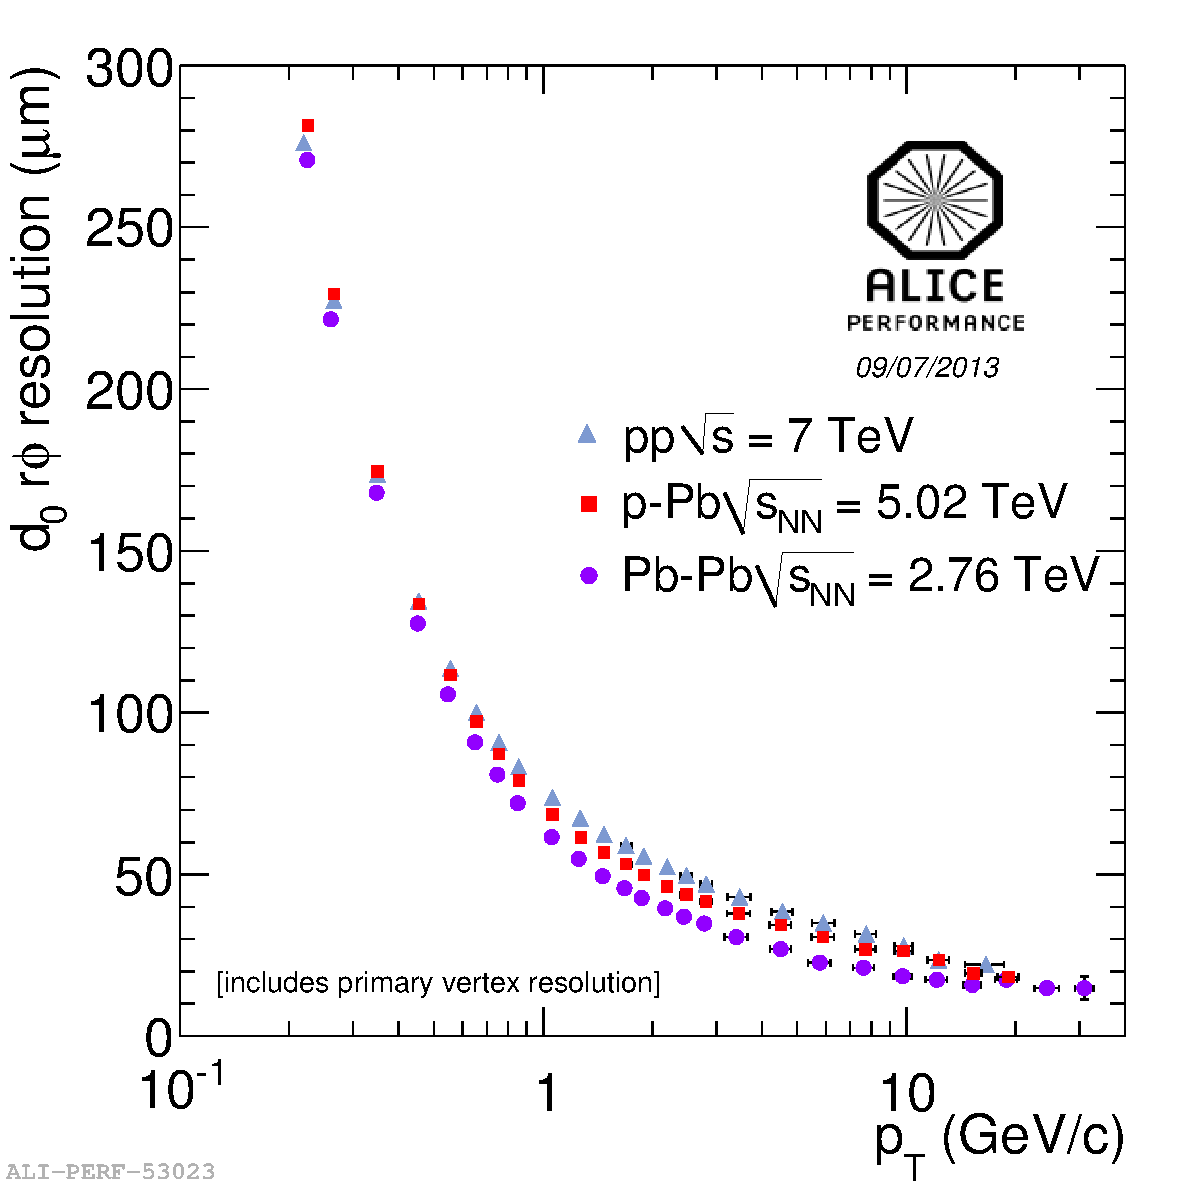
\includegraphics[width=10.cm]{./Version1/FigChapter4/ITSPerformance}
\caption{Track impact parameter resolution in the transverse plane (r$\phi$) vs \pt for charged particle}
\label{fig:itsperformance}
\end{center}
\end{figure}


{\Large\textsl{TPC}}\\
The TPC \cite{cite:TPC} (Figure \ref{fig:tpc}) is the main tracking detector of the central barrel, optimized to provide, together with the other central barrel detectors, charged- particle momentum measurements with good two-track separation, particle identification and vertex determination. The TPC was designed for an excellent tracking performance in the high multiplicity environment of Pb--Pb collisions. For this reason, it was chosen to be a drift chamber, cylindrical in shape, 5 m long, with the inner radius (r$_{in}$ $\sim$ 85 cm) determined by the maximum acceptable track density, and the external one (r$_{ext}$ $\sim$ 250 cm) by the minimum track length for which dE/dx resolution is $<$ 10\%. The TPC volume is filled with 90 m$^{3}$ of Ne/CO$_{2}$/N$_{2}$ (90/10/5). The readout planes are divided in 18 sectors in which multi-wire proportional chambers (with cathode pad readout) are housed. Because of its good d$E$/d$x$ resolution, the TPC can identify particles with \pt $<$ 1 GeV/$c$ on a track-by-track basis. 

\begin{figure}[htbp]
\begin{center}
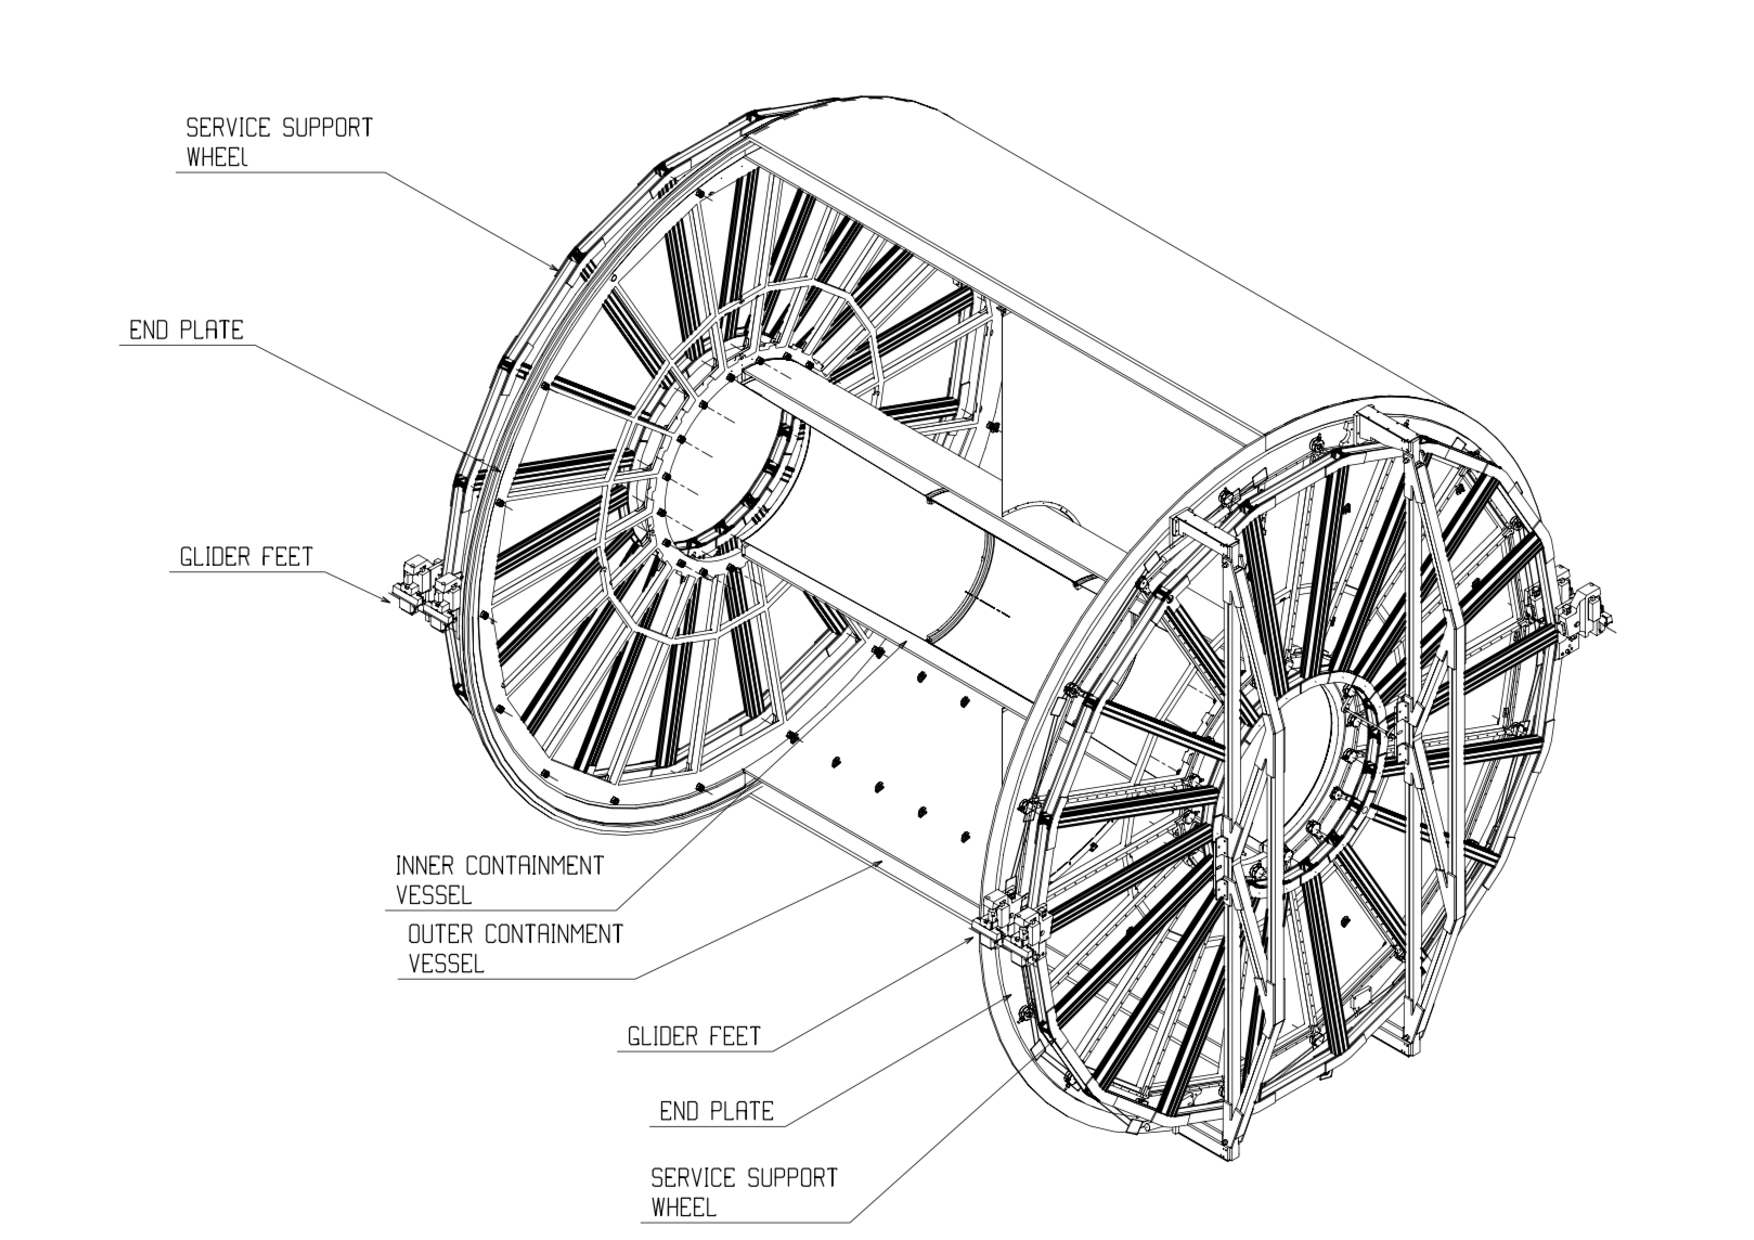
\includegraphics[width=10.cm]{./Version1/FigChapter4/FigureTPC}
\caption{Schematic view of the TPC}
\label{fig:tpc}
\end{center}
\end{figure}

Charged particles traveling through the TPC ionize the detector?s gas; the measurement of this loss of energy is what we need to identify a particle. The physics observable in this case is the energy loss per unit length, within the matter crossed by the charged particle, which we call specific energy loss, also denoted by dE/dx. This is described by the Beth--Bloch equation, \ref{eq:BB}, that highlights the key of the identification technique: this observable depends only on the charge and on velocity ($\beta$) of the particle, which, in turn, depends only on the momentum and the mass of the ionizing particle. Since momentum is already known due to track curvature and charge is unitary for most measured tracks, measuring the dE/dx allows us to indirectly determine mass and thus determine the particle species.
The Bethe-Bloch equation gives the mean specific energy loss:
\begin{equation}\label{eq:BB}
- \langle\frac{dE}{dx}\rangle = k_{1} \cdot z^{2} \frac{Z}{A} \cdot \frac{1}{\beta^{2}}[\frac{1}{2}ln(k_{2}\cdot m_{e}c^{2}\cdot \beta^{2} \gamma^{2})-\beta^{2}+k_{3}]
\end{equation}

where $\beta\gamma$ = $\ensuremath{p}$/Mc and:
Z: atomic number of the ionized gas (in this case Ne/CO$_{2}$/N$_{2}$)\\
A: mass number of the ionized gas (g/mol)\\
m$_{e}$: electron mass\\
z: electric charge of the ionizing particle in unit of electron charge e\\
M: ionizing particle mass\\
$\ensuremath{p}$: ionizing particle momentum\\
$\beta$: ionizing particle velocity normalized to the light velocity c\\
$\gamma$ = 1/$\sqrt{1-\beta^{2}}$, Lorent factor\\
k$_{1}$, k$_{2}$, k$_{3}$: constants depending on the ionized medium\\ 


For a given ionizing particle mass hypothesis, a given momentum and a given length of the trajectory in the ionizing medium, the total charge deposited along the trajectory is subject to statistical fluctuations. This random variable follows a Landau distribution, that give us the opportunity to measure the mean value hdE/dxi. The long tail of the Landau distribution is usually truncated at 50\%-70\% of the collected signal. 

\begin{figure}[htbp]
\begin{center}
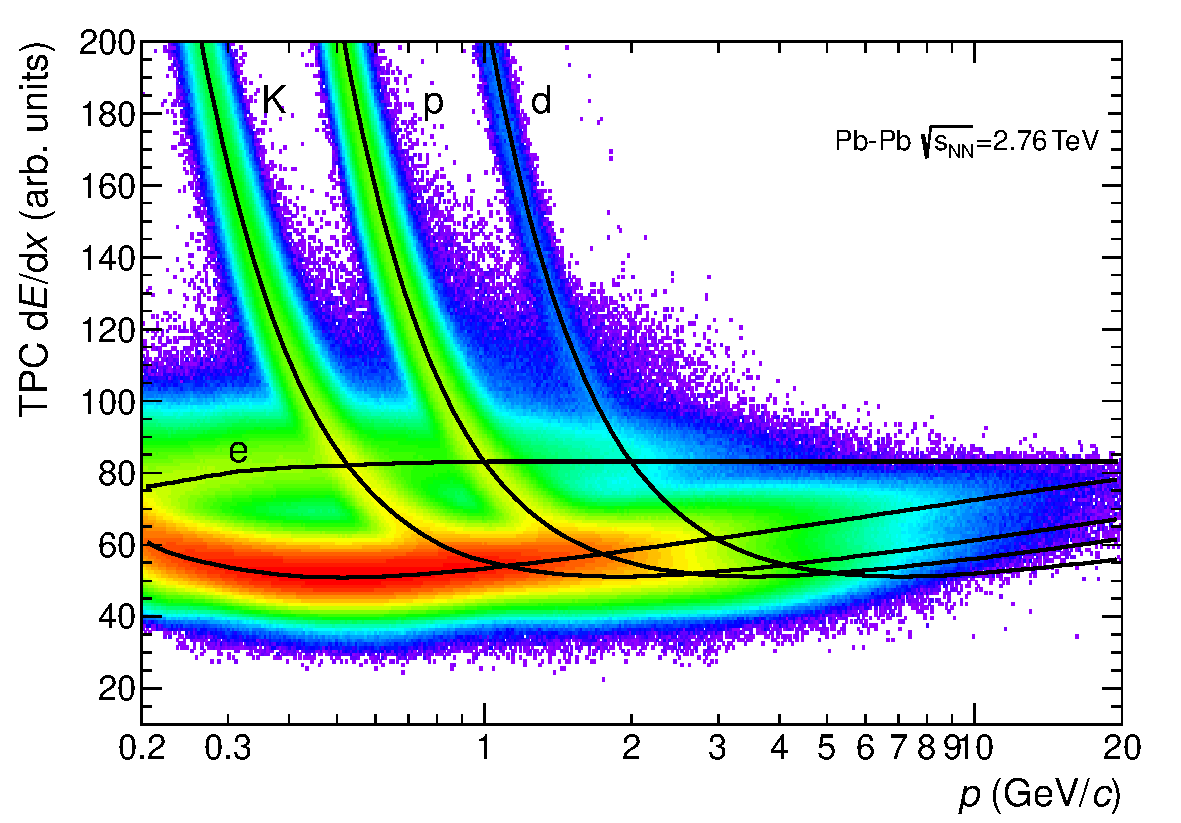
\includegraphics[width=10.cm]{./Version1/FigChapter4/TPCPID}
\caption{Specific energy loss (d$E$/d$x$) in the TPC vs. particle momentum in Pb--Pb collisions at \snn= 2.76 TeV. The lines show the parametrisations of the expected mean energy loss.}
\label{fig:tpcpidPbPb}
\end{center}
\end{figure}


The specific energy loss in the TPC as a function of momentum is shown in Figure \ref{fig:tpcpidPbPb}. The different bands characteristic for e$^{\pm}$, $\pi^{\pm}$, K$^{\pm}$, p$^{\pm}$ are clearly visible. These are the evidence of the statistical distribution of the measured energy loss around the expected mean value. The expected value correspond to the prediction by a Bethe--Bloch experimental parametrization (superimposed as black lines in the Figure). For a track within the TPC the relevant quantity to be considered for PID is the difference between the measured specific energy loss and the corresponding predicted value, by the Bethe-Bloch parametrization for a given measured momentum. If normalized to the resolution of the d$E$/d$x$ measurement in the TPC, this difference could be expressed in number of $\sigma$(see Equation \ref{eq:nsigma}). In this way it is possible to estimate more quantitatively the goodness of a mass hypothesis. This also gives us the possibility to choose the strictness we want to adopt in the identification of a particle (n$_{\sigma}$ , n = 2, 3, 4):

\begin{equation}\label{eq:nsigma}
n_{\sigma} = \frac{(dE/dx)_{measured}-(dE/dx)_{Bethe-Bloch}}{\sigma_{TPC}}
\end{equation}


{\Large\textsl{V0}}\\
The VZERO detector \cite{cite:V0} consists of two segmented arrays of plastic scintillator counters, called VZERO-A and VZERO-C, placed around the beam-pipe on either side of the IP: one at Z = 340 cm, covering the pseudo-rapidity range [2.8; 5.1], and the other at Z = -90 cm (in front of the absorber), covering the pseudo-rapidity range [-3.7; -1.7]. They consist of 32 counters distributed in four rings, each divided in eight 45  sectors. Each counter is made of scintillator material embedded with WaveLength Shifting fibers. Clear fibers collect and transport the signal to photomultipliers 3 - 5 m far from the detector, inside the L3 magnet. The counters have a time resolution better than 1 ns. Their response is recorded in a time window of 25 ns around the nominal beam crossing time.
The VZERO has an important role in rejecting background from beam-gas collisions (see, Figure \ref{fig:v0}) exploiting the relative time-of-flight measurement between the two arrays: when the beam-gas collision takes place outside the region between the two arrays, particles arrive 6 ns before or after the time of a beam-beam collision.

\begin{figure}[htbp]
\begin{center}
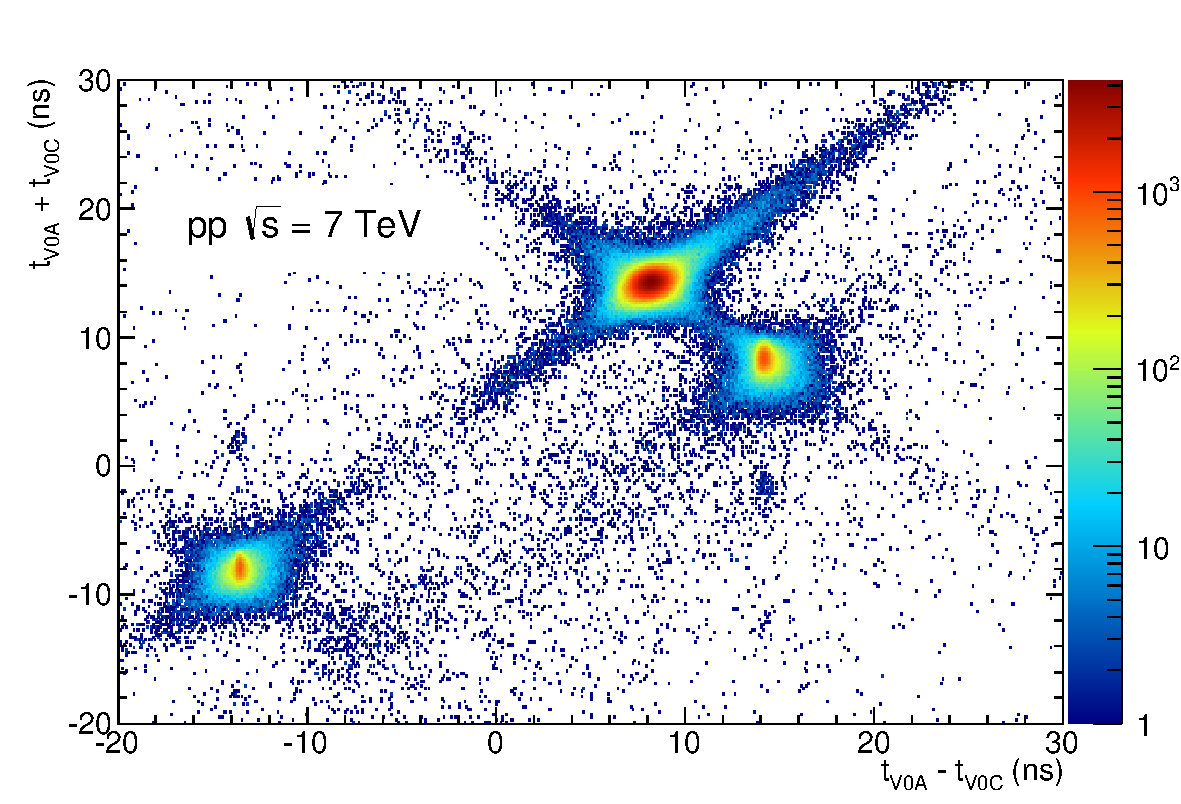
\includegraphics[width=10.cm]{./Version1/FigChapter4/FigureV0}
\caption{Correlation between the sum and difference of signal times in V0A and V0C. Three classes of events collisions at (8.3 ns, 14.3 ns), background from Beam 1 at (-14.3 ns, -8.3 ns), and background from Beam 2 at (14.3 ns, 8.3 ns) can be clearly distinguished.}
\label{fig:v0}
\end{center}
\end{figure}

The VZERO is a trigger detector that will provide a minimum-bias trigger for all colliding systems to the central barrel detectors and three centrality triggers in p--Pb and Pb--Pb collisions (multiplicity, central and semi-central).  

The first parameter to be determined in A--A(p--A) collisions is the centrality(multipliciy). This is defined according to the value of the impact parameter, b, and provides a geometrical scale of the overlapping region between the colliding nuclei: a collision will be defined from central to peripheral, as the impact parameter increases. The centrality of a collision is not directly available and must be deduced from a combination of experimentally measured quantities and Monte Carlo simulations.
There are a number of observables that can be measured and used as centrality estimators. The charged-particle multiplicity N$_{ch}$ and the transverse energy E$_{\mathrm{T}}$ measured around mid-rapidity are measurable quantities related to the energy deposited in the interaction region (these are therefore related to N$_{part}$). These variables increase significantly increasing the centrality of the collisions. Another measurable quantity to estimate the centrality is the zero-degree energy EZDC, namely the energy carried by spectator nucleons N$_{spec}$ = 2A - N$_{part}$ = E$_{ZDC}$/E$_{A}$, where E$_{A}$ is the beam energy per nucleon.
Typically a measured distribution of one of the previous observables is mapped to the corresponding distribution obtained from phenomenological Glauber calculations. The Glauber model \cite{cite:glauber,cite:glauber1} uses a semi-classical approach: the A?A collision is assumed to be an incoherent superposition of N elementary nucleon- nucleon collisions. The main parameters of the model are the inelastic nucleon- nucleon collision cross-section  $\sigma_{n}$ and the nuclear density distribution $\rho$(r). In practice, the simulated distribution well reproduce the measured distribution or the latter is fitted with an analytical function. The experimental distribution can then be divided in classes with sharp cuts on the measured observable (E$_{ZDC}$, E$_{T}$ or N$_{ch}$). These "centrality" classes will correspond to well defined percentage of the integral of the distribution. A given centrality class in the measured distribution, corresponds to the same class in the simulated distribution, where the main geometrical variables (N$_{part}$, N$_{coll}$ and T$_{AA}$) can be determined. The number of classes that can be defined depends on the resolution achievable on the selection variable.
In the analysis described in this thesis the centrality(multiplicity) estimation is based on the measurement of the multiplicities from the VZERO scintillators \cite{cite:centralitypPb}\cite{cite:centralityPbPb}. This is the method that achieve the best centrality resolution: it ranges from 0.5\% in central to 2\% in peripheral collisions. Other methods, as the ones based on the E$_{ZDC}$ measurement or based on the estimate of the number of tracks in the SPD or TPC, are used to asses a systematic uncertainty on the centrality determination.
The distribution of the VZERO amplitudes is shown in Figure \ref{fig:centralityestimate} where the centrality(multiplicity) percentiles are also indicated. 

\begin{figure}[htbp]
\begin{center}
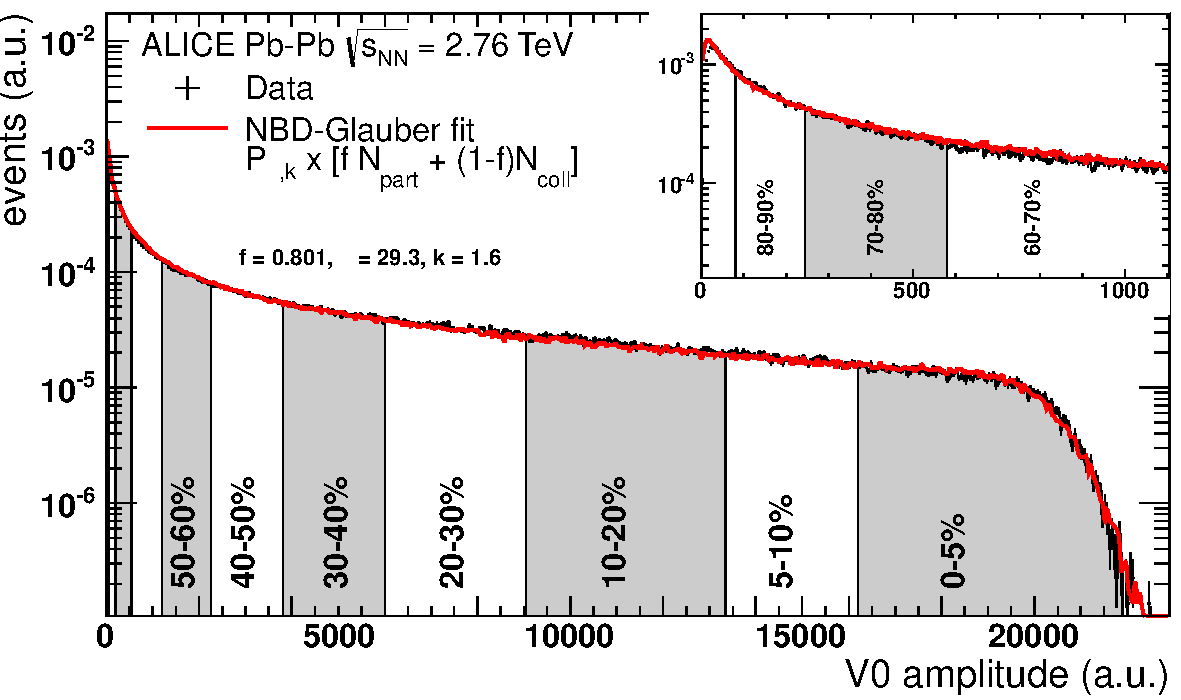
\includegraphics[width=12.cm]{./Version1/FigChapter4/CentralityPbPb}
\hspace{1.0cm}
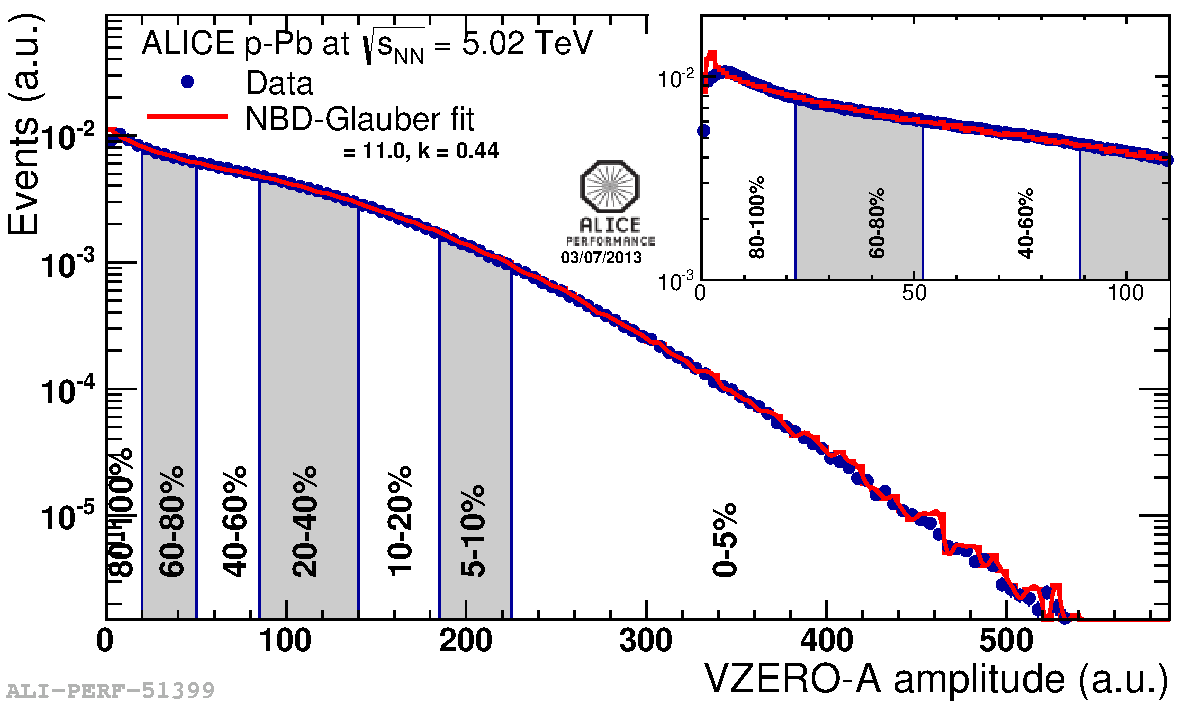
\includegraphics[width=12.cm]{./Version1/FigChapter4/CentralitypPb}
\caption{Distribution of the V0 amplitude (sum of V0A and V0C in top, V0A in bottom). The inset shows a magnified version of the most peripheral region.}
\label{fig:centralityestimate}
\end{center}
\end{figure}

\newpage
\subsubsection{Data Acquisition (DAQ) and trigger system}\label{label:aliceDAQ}
The architecture of data acquisition is shown in Figure \ref{fig:daq}. The tasks of the ALICE DAQ system are the assembly of event informations from individual detectors into complete events (event building) as well as buffer- ing and export of assembled events to permanent storage. The DAQ is designed to process a data rate up to 1.25 GB/s in heavy-ion runs. Event building is done in two steps. Data from the detectors is received by Detector Data Links (DDLs) on Local Data Concentrators (LDCs). The LDCs assemble the data into sub-events that are then shipped to Global Data Collectors (GDCs). A GDC re- ceives all sub-events from a given event and assembles them into a complete event. These events are subsequently stored on a system called Transient Data Storage (TDS).

\begin{figure}[htbp]
\begin{center}
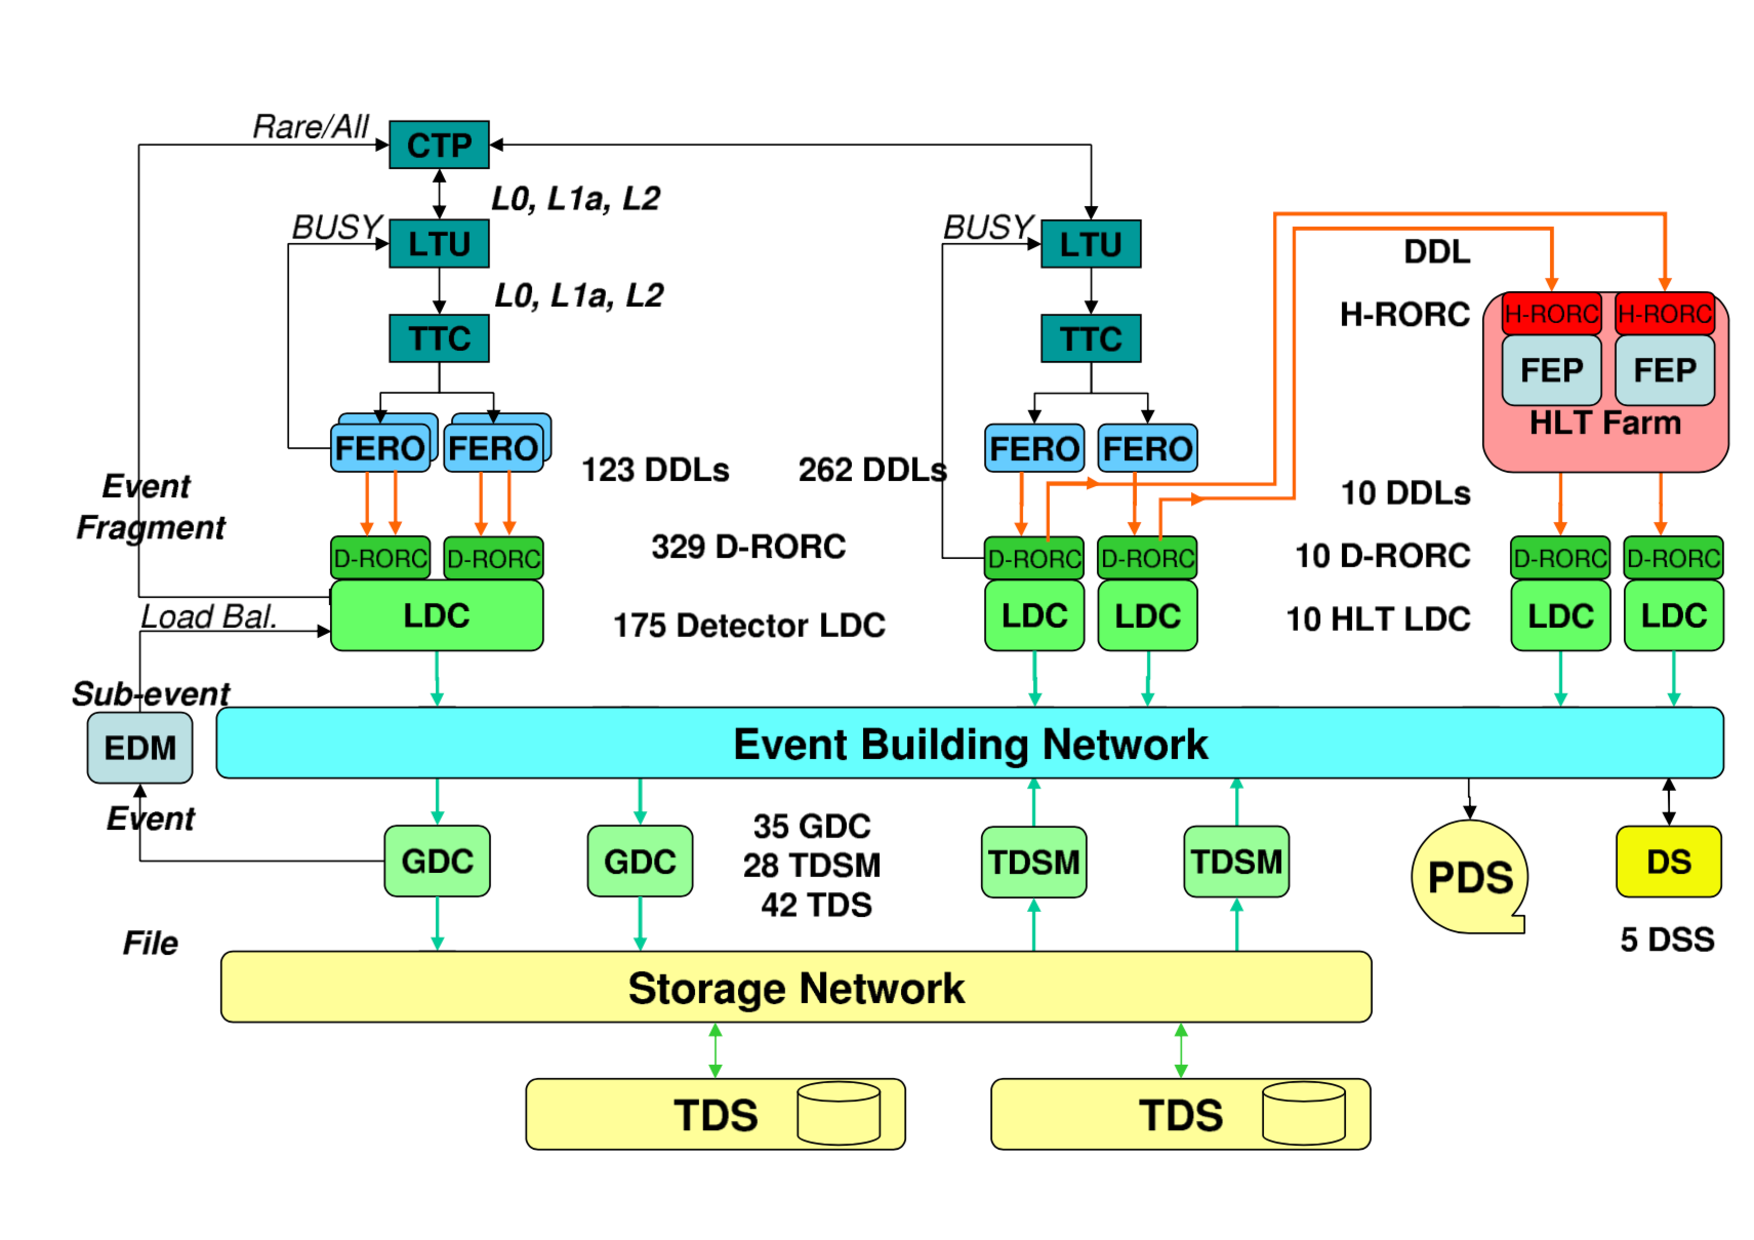
\includegraphics[width=14.cm]{./Version1/FigChapter4/FigureDAQ}
\caption{The overall architecture of the ALICE DAQ and the interface to the HLT system.}
\label{fig:daq}
\end{center}
\end{figure}

 ALICE can simultaneously take data in several partitions, where a set of detec- tors can store their outputs. Since a partition is a group of commonly controlled detectors, a given detector can only be active in one partition at a time. The ac- tive detectors in a given partition may be assigned to data taking groups called clusters, for which triggers can be defined. Therefore, upon a trigger only a sub- set of the whole partition may be read out. Furthermore, a triggering detector does not have to be necessarily part of the partition.
ALICE has a two-layer trigger architecture \cite{cite:daq}. The low-level trigger is a hardware trigger called Central Trigger Processor (CTP). The High-Level Trigger (HLT) is implemented as a pure software trigger. The CTP combines inputs from different trigger sources, namely the various detectors. These inputs are single signals, like a hit in the detector, or, can be the result of fast calculation performed directly in the detectors. The HLT allows the implementation of sophisticated logic for the triggering. In contrast to the CTP which governs the readout of the detectors, the HLT receives a copy of the data read out from the detectors and processes them.
The hardware trigger combines the trigger signals of the various detectors to decide if an event is accepted, that means it is read out and written to disk. Several trigger levels reduce the event rate depending on the input signals. The first level, called L0, is delivered after 1.2 ?s, while the second, called L1, after 6.5 ?s. The final trigger, L2, is delivered after 100 ?s, upon completion of the drift time in the TPC. Only after an L2 trigger the event is finally stored. The rates of different trigger classes are very different. By definition minimum-bias triggers have the highest rate; other triggers that look for rare signals are characterized by much lower rates. In order to cope with different scenarios, downscaling factors can be applied to the trigger classes individually, i.e. only every nth event fulfilling the trigger condition is read out. The total recording rate is limited by the maximum bandwidth of data that can be recorded to disk and tape.
The ALICE software trigger, called HLT, is a farm of multiprocessor computers. The aim is to have about 1000 PCs processing the data in parallel allowing an online analysis of the events. A trigger decision comes from the analysis of a more comprehensive set of information than what happens for the hardware trigger, giving the possibility to apply more sophisticated triggers. Examples include triggers on high energy jets or on muon pairs. Furthermore, the HLT can significantly reduce the event size by selecting regions of interest (partial readout of detectors) and by further compression of the data. The HLT receives a copy of the raw data and performs per detector reconstruction, partly aided by hardware coprocessors. Subsequently, the trigger decision is based on the global reconstructed event. In the same step a region of interest can be selected. In the last optional step, if the trigger decision is positive, the data are compressed. The trigger decision, partial readout information, compressed data, and the re- construction output is sent to LDCs and subsequently processed by the DAQ. In terms of the overall DAQ architecture, data sent by HLT is treated like stemming from a detector.

\newpage
\subsubsection{ALICE offline software frame work}\label{label:alicesw}
The required computing resources for the reconstruction and analysis of the raw data as well as the production of simulated events needed for the understanding of the data exceed the computing power of single institutes and even centers like CERN. Therefore, institutes that are part of the Collaboration also provide storage and computing resources. Distribution of the data for reconstruction and analysis cannot be performed manually and this led to the need for an automated system. The concept of a decentralized computing model called Grid \cite{cite:grid} was identified as a solution.\\


{\Large\textsl{The AliEn Framework}}\\
The Grid paradigm implies the unification of resources of distributed computing center, in particular computing power and storage, to provide them to users all over the World. It allows computing center to offer their resources to a wider community and the local resources to be shared by an entire collaboration.
Software that implements the Grid concept is called Grid middleware. ALICE has developed a Grid middleware called AliEn \cite{cite:alien} since 2001. An ALICE user employs AliEn to connect to the ALICE Grid which is composed of a combination of general services that are provided by many Grid middleware solutions and ALICE-specific services provided by AliEn. Parts of the ALICE Grid are: i) a global file catalog that is a directory of files in storage elements distributed over the Globe, ii) the automatic matching of jobs for execution to a suitable location in one of the connected sites, iii) a shell-like user interface and iv) API9 services for the ROOT framework \cite{cite:aliroot}.\\


{\Large\textsl{AliRoot Framework}}\\
AliRoot \cite{cite:ALICE} is the offline framework for simulation, alignment, calibration, reconstruction, visualization, quality assurance, and analysis of experimental and simulated data. It is based on the ROOT framework. Most of the code is written in C++ with some parts in Fortran that are wrapped inside C++ code. Re-usability and modularity are the basic features of the AliRoot framework. Modularity allows parts of the code to be replaced, with minimum or no impact on the rest (for example changing the event generator, the transport Monte Carlo or the reconstruction algorithms). This is achieved implementing abstract interfaces. In addition codes for each detector subsystem are independent modules with their specific code for simulation and reconstruction and the code can be developed concurrently with minimum interference. Re-usability is meant to maintain a maximum amount of backward compatibility as the system evolves.

\begin{figure}[htbp]
\begin{center}
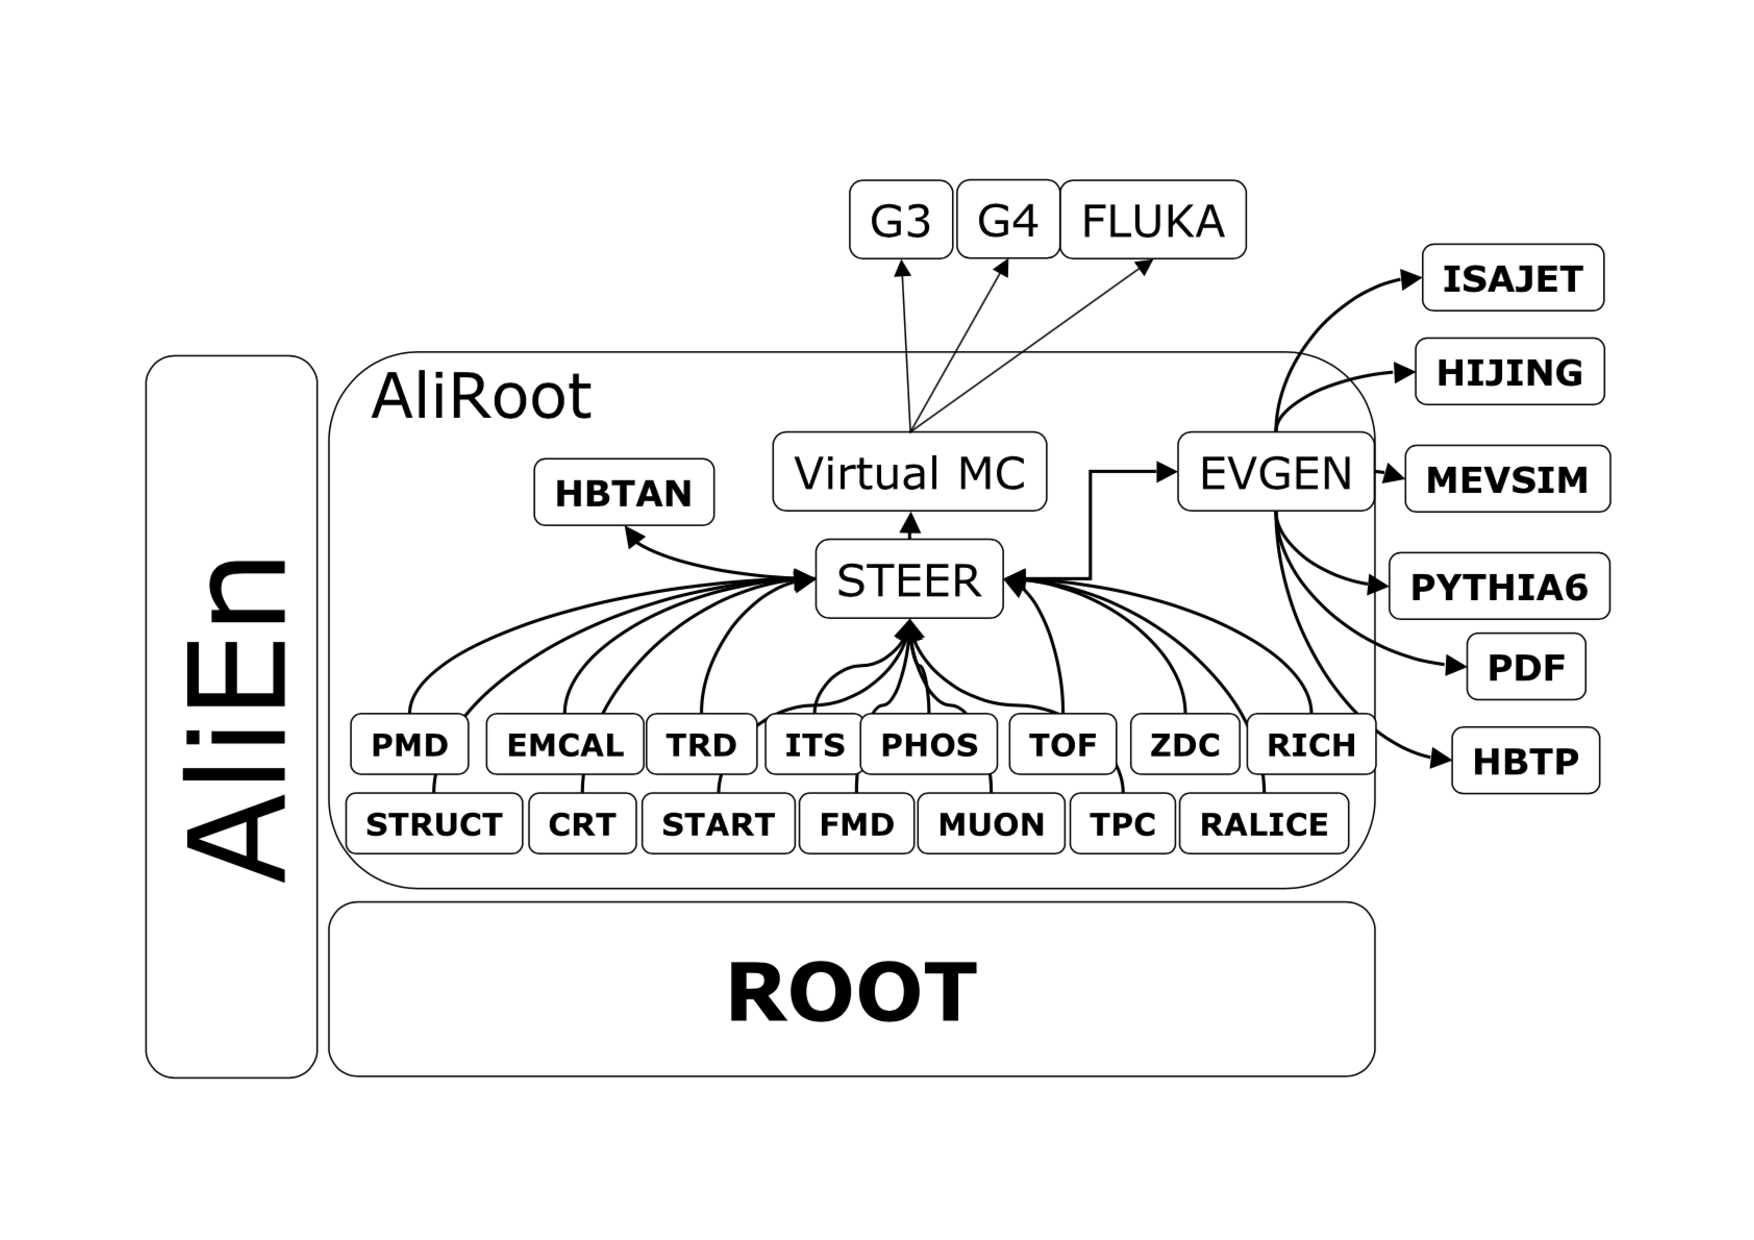
\includegraphics[width=16.cm]{./Version1/FigChapter4/FigureAliRoot}
\caption{Schematic view of the AliRoot framework}
\label{fig:aliroot}
\end{center}
\end{figure}

The central module of the AliRoot framework is STEER (Figure \ref{fig:aliroot}) which provides several common functions such as: steering of program execution for simulation, reconstruction and analysis; general run management, creation and destruction of data structures, initialization and termination of program phases; base classes for simulation, event generation, reconstruction, detectors elements.
For event simulation the framework provides the following functionality:

\newpage
